\documentclass[11pt]{book}

% Use the ETAMU physics style package
\usepackage{../../shared/styles/etamu-physics}

% Document metadata
\title{University Physics I\\Instructor Manual}
\author{ETAMU Physics Department}
\date{\today}

\begin{document}

\frontmatter
\maketitle

\tableofcontents
\listoffigures

\chapter{Preface}

Welcome to the Level 1 Physics Instructor Manual. This manual provides comprehensive coverage of introductory physics topics with detailed solutions, teaching notes, and extensive LaTeX examples for creating professional physics documents.

\section{How to Use This Manual}

This manual is designed to:
\begin{itemize}
    \item Provide complete solutions to all problems
    \item Demonstrate best practices for typesetting physics content
    \item Include LaTeX tutorials throughout for common physics elements
    \item Serve as a template for creating additional course materials
\end{itemize}

\section{LaTeX Resources}

Throughout this manual, you'll find tutorial boxes that explain how to create various elements in LaTeX. These are designed to help you modify and extend the course materials effectively.


\mainmatter

% Include chapters from separate files
\chapter{Momentum and Impulse}

The first section of this class typically covers momentum, impulse, and 
conservation of momentum.  For reference, these three ideas are given below
in mathematical form.

\begin{align}
    \vect{p} &= m\vect{v} \tag{Momentum} \\
    \vect{J} &= \Delta \vect{p} = \vect{F}_{\text{avg}}\Delta t \tag{Impulse} \\
    \sum \vect{p}_{\text{initial}} &= \sum \vect{p}_{\text{final}} \tag{Conservation of Momentum}
\end{align}


\textbf{All} problems in this section can be solved only with the above equations! 
Take careful note that the conservation of momentum condition is a \textit{vector} sum! Also take note
of the impulse equation used here. This form is only valid for a constant force.  Calculus 1
is a co-requisite for this course, so at this point student will likely not be familiar
or comfortable with the idea of an integral.\\

In addition to these equations, you will also need to know how to break vectors into components, 
since we will be dealing with some two-dimensional problems. The most important picture
for knowing how to accomplish this is shown below. \\

\vspace{2em}

\begin{center}
    \begin{tikzpicture}
        \draw[->, >=Stealth, thick] (0,0) -- (4,3) node[midway, above] {$\vect{A}$};
        \draw[->, >=Stealth, thick] (0,0) -- (4,0) node[midway, below] {$A_x = A \cos \theta$};
        \draw[->, >=Stealth, thick] (4,0) -- (4,3) node[midway, right] {$A_y = A \sin \theta$};
        \draw (4,0) -- (4,3) -- (0,0);
        \node at (.7, 0.25) {$\theta$};
        \draw (0.3,0) arc (0:36.87:0.3);
        \node at (2,-2) {Right Triangle Representation of Vector};
        % Draw arc and label phi in the upper right corner
        \draw (4,2.6) arc (-90:-160:0.3);
        \node at (3.75,2.4) {$\phi$};
        \node at (2.3,-0.75) {$=A \sin \phi$};
        \node at (5.5,1) {$=A \cos \phi$};
    \end{tikzpicture}
\end{center}

If you are teaching this course, you will be explaing this diagram \textbf{very} frequently.
Make sure you understand it well, and can explain it clearly to students! We have included a
large format version of this same picture on the first page for easy reference. Trust us, you'll need it. \\ 

\newpage
\section{Momentum Tutorial 1: Oomph}

\textbf{Approximate Time:} 50 minutes \\
\textbf{Equipment Needed:} None \\
\textbf{Pre-Lecture Required?}: No \\

This introductory tutorial is meant to do two things: (1) introduce you to the idea of momentum
and impulse, and (2) get students used to studio mode and working in groups (assuming this is
the first assignment of the semester). \\

The tutorial introduces the concept of momentum under the guise of \textbf{``oomph''} (a non-technical term
for momentum). The students are asked to make qualitative predictions about the oomph of various objects
of different masses and speeds.  Ideally, the students will come to the conclusion that oomph is proportional
to both mass and speed, and that the mathematical expression for oomph is $p = mv$.\\

The second section of the tutorial introduces the idea of impulse, and how a force acting over a time interval
can change an object's momentum.  The students are asked to make qualitative predictions about how the
change in momentum depends on the force applied to an object and how long it is applied for.  Ideally, the students will come to the conclusion
that the change in oomph is proportional to both the force and the time interval, and that the mathematical expression for impulse is
$J = F \Delta t$. \\

At this stage, it is enough that students understand what these two concepts are.  You will note
that none of the equations are written in vector form.  This is intentional, as we will introduce
the vector nature of momentum and impulse in the next tutorial.  For now, we want students
to get comfortable with the concepts in one dimension. \\

\begin{tutorialbox}[title=Student Issue 1: Forces over Time]
A common issue that students have is believing that applying a force
over 5 seconds and applying the same force over 10 seconds both result in the same 
momentum in the end.  It is often because students operate under a sort of "maximum" 
force idea, where they are thinking about \textit{themselves} pushing the object.
Since a person has a maximum force they can apply (and because friction and other things
exist), in reality you can really only speed things you're pushing up to a certain point, 
so time doesn't seem to matter. 
\end{tutorialbox}

\begin{problembox}[title=Learning Outcomes]
\begin{enumerate}[label=(\alph*)]
    \item Momentum is a measure of mass in motion and is calculated by $p = mv$.
    \item Impulse is a measure of an object's \textbf{change} in momentum, and is calculated by \\ $J = F \Delta t = \Delta p$.
    \item Group work and discussions should be written out clearly on whiteboards.
\end{enumerate}
\end{problembox}

\newpage
\section{Momentum Problem Set 1: Impulse in One Dimension}
\textbf{Approximate Time:} 50 minutes \\
\textbf{Equipment Needed:} None \\
\textbf{Pre-Lecture Required?}: Yes - Area under the curve integration\\

Each of these problems can be solved by first finding the impulse, either by using
$J = F \Delta t$ for constant forces, or by finding the area under the curve for variable forces, 
in which cases a graph is provided.\\


\noindent
\textbf{Problem 1:} A 50.0 kg archer, standing on frictionless ice, shoots a 100.0 g 
arrow at a speed of 100.0 m/s. The direction that the arrow travels is defined to 
be the positive direction.
\begin{enumerate}[label=(\alph*)]
    \item What is the sign of the impulse (positive or negative)imparted to the arrow?
    \item What magnitude impulse did the archer impart to the arrow?
    \item Estimate (just make a guess, .1 s, .5 s, 2 s, etc.) how much time the string on the bow was in contact with the arrow.
    \item Calculate the force the bow string imparted on the arrow.
\end{enumerate}
\chapter{Experiment 1}
This is the first experiment chapter. Add your content here.

\section{Energy and Work}

The work-energy theorem states that the work done on an object equals its change in kinetic energy:

\[ W = \Delta KE = \frac{1}{2}mv_f^2 - \frac{1}{2}mv_i^2 \]

\begin{tutorialbox}[title=Creating Energy Diagrams]
Use PGFPlots for energy graphs:
\begin{verbatim}
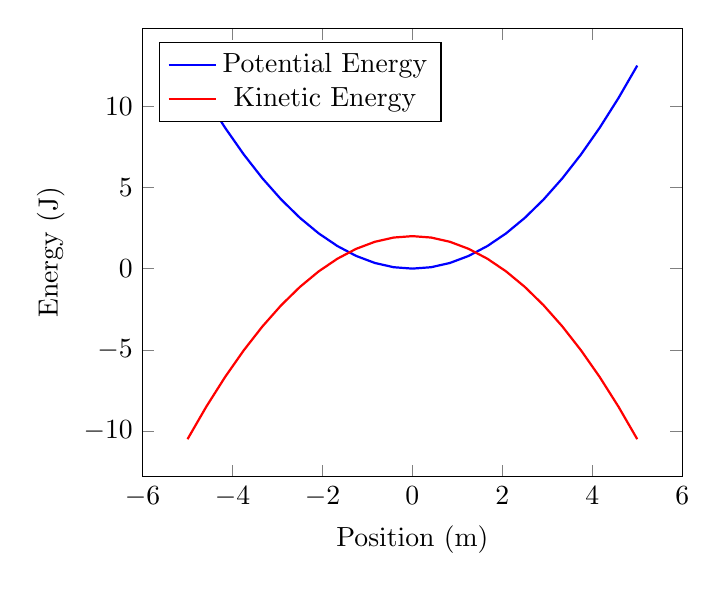
\begin{tikzpicture}
\begin{axis}[
    xlabel={Position (m)},
    ylabel={Energy (J)},
    legend pos=north west
]
\addplot[blue,thick] {x^2/2};
\addlegendentry{Potential Energy}
\addplot[red,thick] {2-x^2/2};
\addlegendentry{Kinetic Energy}
\end{axis}
\end{tikzpicture}
\end{verbatim}
\end{tutorialbox}

\backmatter

\appendix

\chapter{LaTeX Quick Reference}

\section{Common Physics Symbols}
\begin{tabular}{ll}
    \toprule
    Symbol & LaTeX Command \\
    \midrule
    $\vect{F}$ & \texttt{\textbackslash vect\{F\}} \\
    $\uvect{r}$ & \texttt{\textbackslash uvect\{r\}} \\
    $\dv{x}{t}$ & \texttt{\textbackslash dv\{x\}\{t\}} \\
    $\pdv{f}{x}$ & \texttt{\textbackslash pdv\{f\}\{x\}} \\
    $\SI{9.8}{\meter\per\second\squared}$ & \texttt{\textbackslash SI\{9.8\}\{\textbackslash meter\textbackslash per\textbackslash second\textbackslash squared\}} \\
    \bottomrule
\end{tabular}

\section{Useful Packages}
\begin{itemize}
    \item \texttt{physics} - Physics notation and operators
    \item \texttt{siunitx} - SI units and number formatting
    \item \texttt{tikz} - Creating diagrams and figures
    \item \texttt{pgfplots} - Plotting graphs and data
    \item \texttt{circuitikz} - Circuit diagrams
\end{itemize}

\end{document}